\chapter{Objektorientierte Modellierung}

Consetetur sadipscing elitr, sed diam nonumy eirmod tempor invidunt ut labore et dolore magna aliquyam erat, sed diam voluptua. At vero eos et accusam et justo duo dolores et ea rebum. Stet clita kasd gubergren, no sea takimata sanctus est Lorem ipsum dolor sit amet. 

\section{Modelle im Softwareengineering}

Duis autem vel eum iriure dolor in hendrerit in vulputate velit esse molestie consequat, vel illum dolore eu feugiat nulla facilisis at vero eros et accumsan et iusto odio dignissim qui blandit praesent luptatum zzril delenit augue duis dolore te feugait nulla facilisi. Lorem ipsum dolor sit amet, consectetuer adipiscing elit, sed diam nonummy nibh euismod tincidunt ut laoreet dolore magna aliquam erat volutpat.   

\section{Objektorientierung – Einführung}

Ut wisi enim ad minim veniam, quis nostrud exerci tation ullamcorper suscipit lobortis nisl ut aliquip ex ea commodo consequat. Duis autem vel eum iriure dolor in hendrerit in vulputate velit esse molestie consequat, vel illum dolore eu feugiat nulla facilisis at vero eros et accumsan et iusto odio dignissim qui blandit praesent luptatum zzril delenit augue duis dolore te feugait nulla facilisi.   

\section{Die Unified Modeling Language (UML)}

Nam liber tempor cum soluta nobis eleifend option congue nihil imperdiet doming id quod mazim placerat facer possim assum. Lorem ipsum dolor sit amet, consectetuer adipiscing elit, sed diam nonummy nibh euismod tincidunt ut laoreet dolore magna aliquam erat volutpat. Ut wisi enim ad minim veniam, quis nostrud exerci tation ullamcorper suscipit lobortis nisl ut aliquip ex ea commodo consequat.   

\newpage

\section{Objekte und Klassen – Modellierung von Realwelt-Zusammenhängen}

% 3.4.1 Objekt vs. Klasse 
\subsection{Objekt vs. Klasse}

Der Objektbegriff in der Softwareentwicklung umfasst Dinge, die man sehen und/oder anfassen kann, wie zum Beispiel eine Katze, einen Tisch, eine Person oder einen Stern, aber auch immaterielle Dinge, wie zum Beispiel ein Konto, eine Reise oder eine Vorlesung. In der objektorientierten Softwareentwicklung werden die (zukünftigen) Objekte\marginpar{Objekt} eines Softwaresystems von Objekten der Realwelt abgeleitet. Abhängig vom Einsatzzweck der Software werden bei der Bestimmung der systeminternen Objekte bestimmte Eigenschaften der Realwelt-Objekte berücksichtigt und andere ignoriert, so dass nur die für die zukünftige Software relevanten Eigenschaften der Realwelt-Objekte betrachtet werden. System-Objekte sind damit Abstraktionen von Realwelt-Objekten.

Ein System-Objekt hat eine eindeutige Identität, die es von anderen Objekten des Systems unterscheidbar macht. Es verfügt über Eigenschaften, kann wechselnde Zustände annehmen und bietet anderen Objekten eine Menge an Operationen an. In Reaktion auf den Aufruf seiner Operationen zeigt das Objekt ein bestimmtes Verhalten. Dabei kann es sich zum Beispiel um die Änderung seines Zustandes oder den Aufruf weiterer (eigener oder fremder) Operationen handeln. In der UML werden Objekte als rechteckige Kästen dargestellt, die (mindestens, s.u.) den Objektnamen\footnote{Der Objektname ist nicht gleichzusetzen mit der Identität des Objektes. Der Name ist lediglich ein Bezeichner, der das Objekt innerhalb eines Diagramms identifiziert, aber nicht im gesamten System.} enthalten (Abb.~\ref{fig:Abb-3-2}).
\begin{wrapfigure}{o}[70pt]{0.6\textwidth}
	%\vspace{-10pt}
	\centering 
	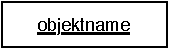
\includegraphics{../grafiken/Kapitel-3/Abb-3-2.pdf}
	\caption{Ein Objekt in UML-Darstellung}
	\label{fig:Abb-3-2}
	\vspace{-6pt}
\end{wrapfigure}
Nach UML-Konvention wird der Objektname unterstrichen dargestellt. Üblich – obwohl die UML diesbezüglich keine Vorgaben macht – ist außerdem, dass Objektnamen mit einem Kleinbuchstaben beginnen und zentriert dargestellt werden. Innerhalb eines Diagramms müssen die Objektnamen eindeutig gewählt werden. Sollten innerhalb eines Diagramms trotzdem zwei Kästchen denselben Namen enthalten – die UML verbietet dies nicht – so ist per Definition mit beiden Kästchen dasselbe Objekt gemeint. Die Darstellung als zwei Kästchen wird vor allem in handschriftlich erstellten Diagrammen aus Lesbarkeitsgründen verwendet.

\begin{wrapfigure}{o}[70pt]{0.6\textwidth}
	%\vspace{-10pt}
	\centering 
	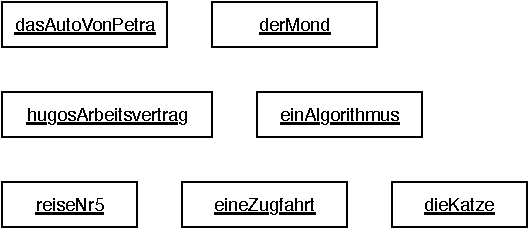
\includegraphics{../grafiken/Kapitel-3/Abb-3-3.pdf}
	\caption{Einige Objekte}
	\label{fig:Abb-3-3}
	\vspace{-6pt}
\end{wrapfigure}
Abbildung~\ref{fig:Abb-3-3} zeigt einige Objekte in UML-Darstellung.
Bei manchen wird aus dem Namen (relativ) deutlich, welches konkrete Realwelt-Objekt sie abbilden sollen. So ist \texttt{dasAutoVonPetra}, sofern man Petra kennt und sie nicht mehr als ein Auto besitzt, einem konkreten Realwelt-Auto zuordenbar. Für \texttt{reiseNr5} bedarf es dagegen schon der zusätzlichen Kenntnis des Kontextes (z.B. die Auflistung von Reisen in einem Katalog), um eine Realwelt-Reise mit diesem Namen zu verbinden. Für Objekte wie \texttt{einAlgorithmus} oder \texttt{eineZugfahrt} und auch \texttt{dieKatze} schließlich lassen sich die gemeinten Realwelt-Entsprechungen nicht bestimmen. Zumindest könnte man anhand der Namen der Objekte aber vielleicht auf die Art des Realwelt-Objektes schließen. So sollte es sich bei \texttt{dieKatze} doch wohl um eine Katze und nicht um einen Hund handeln.


Doch vielleicht trägt mein Meerschweinchen – aus welchem Grund auch immer – den Namen \texttt{dieKatze} und meine Katze heißt stattdessen \texttt{pünktchen}. \begin{wrapfigure}{o}[70pt]{0.7\textwidth}
	%\vspace{-10pt}
	\centering 
	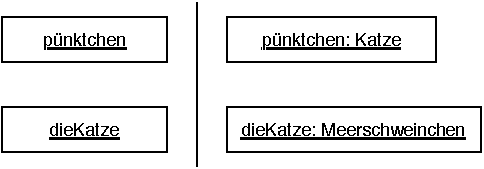
\includegraphics{../grafiken/Kapitel-3/Abb-3-4.pdf}
	\caption{Links: Ein Objekt namens \texttt{pünktchen} und ein Objekt namens \texttt{dieKatze}. Rechts: Ein Katzen-Objekt namens \texttt{pünktchen} und ein Meerschweinchen-Objekt namens \texttt{dieKatze}}
	\label{fig:Abb-3-4}
	\vspace{-6pt}
\end{wrapfigure}
Um solche Sachverhalte unmissverständlich zu modellieren, wird neben dem Objektnamen noch die Information benötigt, um welche Art von Objekt es sich handelt. In der UML-Darstellung eines Objektes wird dafür der Objektname um die Angabe des Namens der so genannten Klasse ergänzt (Abb.~\ref{fig:Abb-3-4} rechts). Die Objektdarstellung ohne zusätzlichen Klassennamen (wie in Abb.~\ref{fig:Abb-3-2} und Abb.~\ref{fig:Abb-3-3}) ist nach UML-Regeln zulässig, sollte aus semantischen Gründen aber nur dann verwendet werden, wenn aus dem Kontext eindeutig auf den Typ (die zugehörige Klasse) des Objektes geschlossen werden kann.

Das Konzept der Klasse\marginpar{Klasse} ist ein wichtiger Bestandteil der objektorientierten Softwareentwicklung.\footnote{Auch wenn es einige wenige objektorientierte Programmiersprachen gibt (z.B. Javascript, Go), die keine Klassen, sondern nur Objekte kennen.} Aus einer konzeptuellen Sicht gruppiert eine Klasse eine Menge von System-Objekten anhand identifizierter Gemeinsamkeiten. So können zum Beispiel alle System-Objekte, die Realwelt-Katzen modellieren, der Klasse Katze zugeordnet werden, während System-Objekte, die Realwelt-Meerschweinchen abbilden, zur Klasse Meerschweinchen gehören. Eine Klasse definiert, welche Aspekte der Objekte für ihre Zugehörigkeit zur Klasse relevant sind. So könnte es zum Beispiel notwendig sein, dass ein Objekt schnurren kann, um vom Typ Katze zu sein, wogegen es irrelevant ist, welche Farbe das Fell hat oder vielleicht auch, ob das Objekt überhaupt ein Fell hat (Nacktkatzen). Klassen sind somit Abstraktionen von System-Objekten. Sie abstrahieren von der konkreten Ausprägung der Eigenschaften ihrer Objekte (z.B. Farbe des Fells) und den Zuständen, in denen sich ihre Objekte befinden können. Aus Implementierungssicht sind Klassen Schablonen für die Erstellung von System-Objekten. Eine Klasse definiert, welche Eigenschaften, welches Verhalten und welche Beziehungen zu anderen Objekten die ihr zugehörigen Objekte aufweisen sollen. Eine Klasse definiert außerdem einen Mechanismus – in der objektorientierten Programmierung als Konstruktor bezeichnet – über den neue Objekte vom Typ der Klasse erzeugt werden können. Jedes zur Laufzeit der Software benötigte Objekt einer Klasse wird so anhand der Vorgaben der Klasse konstruiert.

Diese Erzeugung neuer Objekte einer Klasse nennt man Instanziierung und statt vom Objekt der Klasse spricht man in diesem Zusammenhang von der Instanz der Klasse. Einen inhaltlichen Unterschied zwischen den Begriffen Instanz und Objekt gibt es nicht. Der Begriff Instanz wird verwendet, wenn die Zugehörigkeit eines Objektes zu seiner Klasse wichtig ist („Eine Instanz der Klasse Katze“), weil damit zum Beispiel ausgedrückt werden soll, dass dieses konkrete Objekt alle Eigenschaften besitzt, die die entsprechende Klasse definiert hat. Der Begriff Objekt wird in allgemeineren Zusammenhängen verwendet. Eine scharfe Trennlinie gibt es aber nicht. Letztendlich können die Begriffe synonym verwendet werden – und werden sie in der Literatur auch häufig. Die Menge aller zu einem Zeitpunkt existierenden Instanzen einer Klasse bezeichnet man mit dem Begriff der Extension. 

Die UML-Darstellung einer Klasse ist sehr ähnlich zu der Darstellung eines Objektes. Es handelt sich ebenfalls um ein Rechteck, in dem (mindestens, s.u.) der Klassenname eingetragen ist.
\begin{wrapfigure}{o}[70pt]{0.7\textwidth}
	%\vspace{-10pt}
	\centering 
	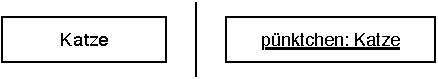
\includegraphics{../grafiken/Kapitel-3/Abb-3-5.pdf}
	\caption{Eine Klasse mit Namen \texttt{Katze} (links) und eine Instanz dieser Klasse mit Namen \texttt{pünktchen} (rechts)}
	\label{fig:Abb-3-5}
	\vspace{-6pt}
\end{wrapfigure}
Abbildung~\ref{fig:Abb-3-5} zeigt eine Klasse \texttt{Katze} und eine Instanz namens \texttt{pünktchen} der Klasse Katze. Im Unterschied zu Objekten wird der Name der Klasse nicht unterstrichen. Zudem ist es üblich, den Klassennamen mit einem Großbuchstaben zu beginnen und ihn zentriert und fett gedruckt zu setzen. Der Klassenname ist üblicherweise ein Substantiv im Singular. Abbildung~\ref{fig:Abb-3-6} zeigt weitere Instanzen der Klasse Katze.

Wichtig ist, dass ausschließlich die Angabe \texttt{:Katze} bestimmt, dass es sich um ein Objekt vom Typ Katze handelt. Der Name des Objektes selber sagt nichts über den Typ des Objektes aus. 
\begin{wrapfigure}{o}[70pt]{0.7\textwidth}
	%\vspace{-10pt}
	\centering 
	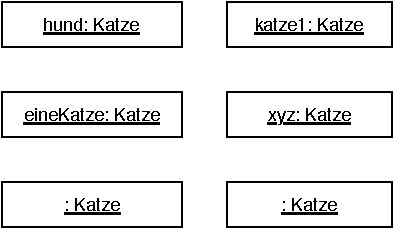
\includegraphics{../grafiken/Kapitel-3/Abb-3-6.pdf}
	\caption{sechs verschiedene Instanzen der Klasse Katze}
	\label{fig:Abb-3-6}
	\vspace{-6pt}
\end{wrapfigure}
So handelt es sich auch bei dem Objekt mit dem Namen \texttt{hund} in Abbildung~\ref{fig:Abb-3-6} um eine Katze. Die beiden unteren Objekte in der Abbildung (\texttt{:Katze}) sind so genannte anonyme Objekte. Diese Form der Darstellung wird verwendet, wenn man nicht eine konkrete, mit einem Namen versehene, Katzen-Instanz modellieren möchte, sondern „irgendein“ Objekt vom Typ Katze. Beachten Sie, dass auch ein anonymes Objekt nur genau \underline{ein} Objekt ist, es steht nicht stellvertretend für alle möglichen Katzen-Instanzen. Im Unterschied zu benannten Instanzen darf es innerhalb desselben Objektdiagramms auch mehrere anonyme Instanzen derselben Klasse geben. Bei diesen handelt es sich dann per Definition um unterschiedliche Objekte. Die beiden anonymen Katzen-Instanzen in Abbildung~\ref{fig:Abb-3-6} modellieren daher zwei unterschiedliche Realwelt-Katzen, bei denen es aber für den Modellierungszweck irrelevant ist, um welche konkreten Realwelt-Katzen es sich handelt. Das Objekt mit Namen \texttt{eineKatze} ist dagegen kein anonymes Objekt sondern modelliert genau diejenige Realwelt-Katze, die den Namen \texttt{eineKatze} trägt.

% 3.4.2 Eigenschaften 
\subsection{Eigenschaften}

Wie schon erwähnt spezifizieren Klassen Eigenschaften, die alle ihre Instanzen besitzen sollen. Dabei werden im Zuge der Abstraktion zwischen Realwelt und Modell nur diejenigen Eigenschaften der zu modellierenden Realwelt-Objekte berücksichtigt, die für den Modellzweck relevant sind. In UML-Notation werden die Eigenschaften in Form von Attributen im Rechteck der jeweiligen Klasse verzeichnet. Dafür wird das Rechteck unterhalb des Klassennamens durch eine Linie horizontal geteilt.
\begin{wrapfigure}{o}[70pt]{0.6\textwidth}
	%\vspace{-10pt}
	\centering 
	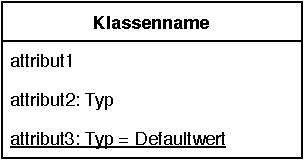
\includegraphics{../grafiken/Kapitel-3/Abb-3-7.pdf}
	\caption{Eine Klasse mit Attributen in UML-Darstellung}
	\label{fig:Abb-3-7}
	\vspace{-6pt}
\end{wrapfigure}
Abbildung~\ref{fig:Abb-3-7} zeigt drei gängige Varianten, wie Attribute innerhalb einer Klasse angegeben werden können.\footnote{Die UML lässt noch weitere Varianten zu.} Wir werden im weiteren Verlauf des Kurses sehen, dass für unterschiedliche Zwecke während des Softwareentwicklungsprozesses unterschiedlich stark detaillierte Klassendiagramme benötigt werden. So wird zum Beispiel in Domänenklassendiagrammen üblicherweise nur der Attributname angegeben, während Klassendiagramme, die auf die Implementierung ausgerichtet sind, die Informationen über Attributtypen und evtl. Vorgabewerte (default values) beinhalten müssen. Sofern Attributtypen in einer Klasse angegeben werden, muss es sich zudem nicht zwangsläufig um programmiersprachliche Datentypen handeln. Gerade in Klassendiagrammen, die für die Kommunikation mit Nicht-Programmierern gedacht sind, finden sich häufiger Angaben wie Euro oder Grad Celsius statt Integer oder Float.

Abbildung~\ref{fig:Abb-3-8} zeigt oben die Klasse \texttt{Auto}, die über die beiden Attribute \texttt{modell} und \texttt{farbe} zwei Eigenschaften von Auto-Objekten spezifiziert.
\begin{wrapfigure}{o}[70pt]{0.8\textwidth}
	%\vspace{-10pt}
	\centering 
	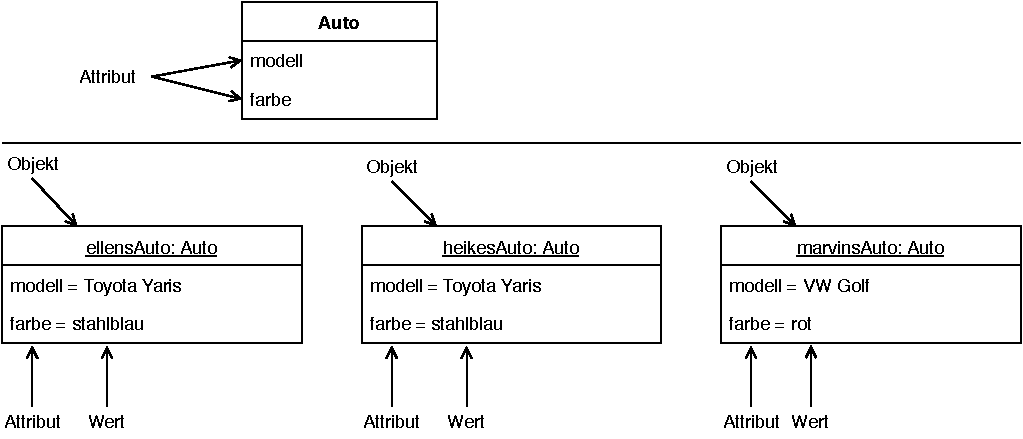
\includegraphics[scale=0.6]{../grafiken/Kapitel-3/Abb-3-8.pdf}
	\caption{Eine Klasse Auto und drei konkrete Instanzen der Klasse}
	\label{fig:Abb-3-8}
	\vspace{-6pt}
\end{wrapfigure}
Die Abbildung zeigt außerdem mit \texttt{ellensAuto}, \texttt{heikesAuto} und \texttt{marvinsAuto} drei konkrete Instanzen der Auto-Klasse, bei denen die Attribute \texttt{modell} und \texttt{farbe} mit konkreten Werten belegt sind. Attribute werden durch die Klasse definiert und sind für jede Instanz vorgegeben. Alle drei Auto-Objekte in Abbildung~\ref{fig:Abb-3-8} beinhalten daher die beiden Attribute \texttt{modell} und \texttt{farbe}. Ein Objekt kann zudem keine Attribute besitzen, die die Klasse nicht vorsieht. So kann zum Beispiel ein konkretes Auto-Objekt keine Angabe über das Baujahr des Autos beinhalten, solange die Klasse Auto ein solches Attribut nicht vorsieht, auch wenn das Realwelt-Auto, das durch das Auto-Objekt abgebildet wird, ein Baujahr besitzt. Die Wertebelegung der vorgegebenen Attribute ist dagegen objektspezifisch und auch veränderlich. So könnte für \texttt{marvinsAuto} die Wertebelegung des Attributs \texttt{farbe} von rot zu grün wechseln, wenn das Auto zum Beispiel neu lackiert wird. Die Änderung der Wertebelegung einer Instanz hat weder Auswirkungen auf ihre Klasse noch auf andere Instanzen derselben Klasse. Die aktuellen Wertebelegungen aller Attribute eines Objektes sowie seine bestehenden Verbindungen zu anderen Objekten (s.u.) bestimmen den so genannten Zustand des Objektes. Daraus ergibt sich, dass sich der Zustand eines Objektes ändert, wenn sich mindestens eine Wertebelegung seiner Attribute ändert. Die Identität eines Objektes ändert sich dagegen niemals. Sie besteht vom Zeitpunkt der Erzeugung bis zur Zerstörung des Objektes, unabhängig davon, wie häufig sich der Zustand des Objektes verändert hat.

Die beiden Auto-Instanzen \texttt{ellensAuto} und \texttt{heikesAuto} stimmen in den Wertebelegungen der Attribute \texttt{modell} und \texttt{farbe} überein. Man bezeichnet Objekte (derselben Klasse), die denselben Zustand aufweisen als zustandsgleich. Zustandsgleiche Objekte sind weiterhin Objekte mit unterschiedlicher Identität! Von der Zustandsgleichheit zu unterscheiden, ist die so genannte referentielle Gleichheit. Referentielle Gleichheit liegt vor, wenn sich hinter zwei unterschiedlichen Objektnamen das identische Objekt verbirgt, es sich also nur um zwei Referenzen auf dasselbe Objekt handelt. Zum Beispiel könnte die Realwelt-Person Henrike Meyer außer über ihren Namen auch über ihre Aliase Bürgermeisterin oder 1.~Vorsitzende des Elternrates bezeichnet werden. Die drei modellierten Objekte zeigen dann nur unterschiedliche Ausschnitte desselben Objektes, nämlich desjenigen Objektes, das die Realwelt-Person Henrike Meyer, die gleichzeitig Bürgermeisterin und 1.~Vorsitzende des Elternrates der Schule ihres Kindes ist, abbildet.

Manche Eigenschaften von Realwelt-Objekten, wie zum Beispiel der Modelltyp eines Autos, ändern sich nicht. Bei der Abbildung einer Eigenschaft auf ein System-Objekt möchte man eine solche Unveränderlichkeit vielleicht auch vorsehen. 
\begin{wrapfigure}{o}[70pt]{0.6\textwidth}
	%\vspace{-10pt}
	\centering 
	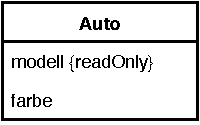
\includegraphics{../grafiken/Kapitel-3/Abb-3-9.pdf}
	\caption{Eine Klasse Auto mit einem unveränderlichen Attribut \texttt{modell} und einem veränderlichen Attribut \texttt{farbe}}
	\label{fig:Abb-3-9}
	\vspace{-6pt}
\end{wrapfigure}
Die UML sieht dafür die Angabe des ergänzenden Merkmals \{readOnly\} vor, die in der Klasse hinter dem Attribut notiert wird, aus Übersichtlichkeitsgründen aber nicht in den einzelnen Objekten (Abbildung~\ref{fig:Abb-3-9}). Die Klasse Auto (und das umgebende Programm) muss dann natürlich später auch so implementiert werden, dass sichergestellt ist, dass jede Auto-Instanz einen Attributwert für \texttt{modell} enthält, dieser Wert aber während der Lebenszeit der Instanz nicht verändert werden kann. In objektorientierten Programmiersprachen ist der Einsatz von Konstanten eine Möglichkeit, die Unveränderlichkeit von Attributwerten zu gewährleisten. Die Angabe von ergänzenden Merkmalen in geschweiften Klammern sieht die UML für verschiedene Zwecke vor und zwar nicht nur in Zusammenhang mit Attributen sondern auch mit Operationen und Beziehungen zwischen Elementen. Wir werden im Laufe des Kurses noch einige von der UML vordefinierte ergänzende Merkmale kennenlernen. Die UML erlaubt darüber hinaus auch benutzerdefinierte ergänzende Merkmale. Im letzteren Fall muss der Ersteller des UML-Diagramms allerdings sicherstellen, dass seine Zielgruppe die Bedeutung der modellierten Ergänzungen versteht.

Bisher haben wir Attribute betrachtet, die zwar durch die Klasse definiert werden, für die aber jede Instanz der Klasse ihre eigenen Wertebelegungen hat. Das Klassenkonzept der Objektorientierung sieht neben solchen Attributen, die auch als Instanzattribute bezeichnet werden, noch eine andere Art von Attributen vor, die so genannten Klassenattribute. 
Ein Klassenattribut ist ein Attribut, das in der Klasse verortet ist und dessen Wert von allen Instanzen der Klasse geteilt wird. Im Unterschied zu Instanzattributen besitzt also nicht jede Instanz eine eigene Wertebelegung für dieses Attribut, sondern es existiert nur ein gemeinsamer Wert. Jede Instanz kann auf das Attribut zugreifen, den Wert des Attributes auslesen und sofern es veränderlich ist, auch den Wert des Attributes ändern. Letzteres sollte bei der konkreten Implementierung geeignet gesteuert werden, da eine durch eine Instanz vorgenommene veränderte Wertebelegung eines Klassenattributes sich auf alle Instanzen der Klasse auswirkt. Klassenattribute verwendet man für die Abbildung von Eigenschaften, die relevant für die inhaltliche Modellierung einer konkreten Klasse sind, sich aber nicht den einzelnen Instanzen der Klasse zuordnen lassen. Ein Klassenattribut existiert auch dann, wenn (noch) keine Instanz der Klasse erzeugt wurde. \begin{wrapfigure}{o}[70pt]{0.8\textwidth}
	%\vspace{-10pt}
	\centering
	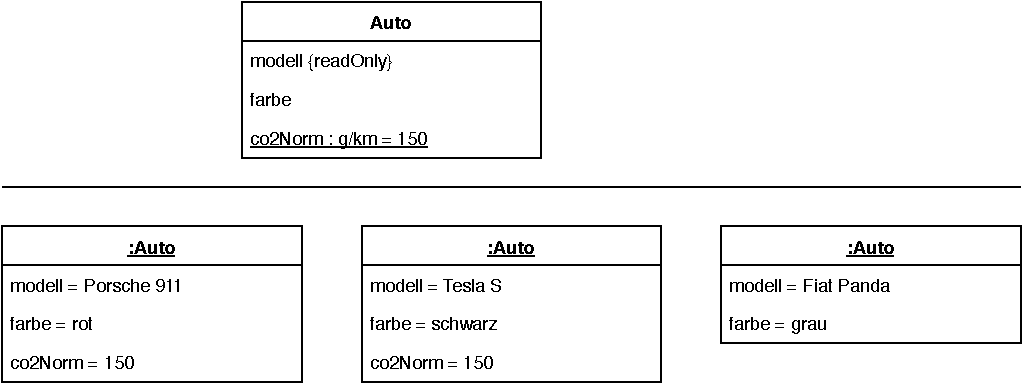
\includegraphics[scale=0.6]{../grafiken/Kapitel-3/Abb-3-10.pdf}
	\caption{Eine Klasse \texttt{Auto} mit Instanzattributen \texttt{modell} und \texttt{farbe} und dem Klassenattribut \texttt{co2Norm} (oben) sowie drei anonyme Instanzen der Klasse Auto (unten)}
	\label{fig:Abb-3-10}
	\vspace{-6pt}
\end{wrapfigure}
Ein Klassenattribut in unserem Autobeispiel-Kontext könnte \texttt{co2Norm} sein, wenn wir idealisiert annehmen, dass für alle Automodelle eine einheitliche CO$_2$-Abgasnorm gilt (Abb.~\ref{fig:Abb-3-10}). Klassenattribute werden in der UML-Darstellung der Klasse unterstrichen. In der Darstellung der Instanzen wird ein Klassenattribut identisch zu den Instanzattributen dargestellt. Häufig werden Klassenattribute aber aus Redundanzgründen (da jede Instanz denselben Wert hat) gar nicht in der Darstellung der Instanzen aufgeführt. Die UML erlaubt es, dass die Angabe der Attribute einer Instanz – nicht nur bezogen auf Klassenattribute sondern auch auf die Instanzattribute – unvollständig ist, weil zum Beispiel nur diejenigen Attribute aufgeführt werden sollen, bei denen noch Diskussionsbedarf besteht.

% 3.4.3 Verhalten
\subsection{Verhalten}

Eine Änderung des Zustands eines Objektes, wie zum Beispiel der schon angesprochene Farbwechsel von Marvins Auto aus Abbildung~\ref{fig:Abb-3-8} von rot zu grün, wird durch die Ausführung von Operationen durchgeführt, die durch die entsprechende Klasse für ihre Instanzen definiert wurden. Operationen spezifizieren, welche Funktionalität ein Objekt (für andere Objekte des Systems) anbietet. Man verwendet in diesem Zusammenhang auch den Begriff Dienstleistung und beschreibt mit den Begriffen Dienstleister und Dienstnutzer, welche Rolle ein Objekt bei Ausführung einer bestimmten Operation einnimmt. Das Objekt, das eine Operation aufruft, ist der Dienstnutzer und das Objekt, dessen Operation aufgerufen wird, ist der Dienstleister. Die entsprechende Operation (bzw. die Funktionalität, die sie abbildet) ist dementsprechend der Dienst. Die reine objektorientierte Modellierung abstrahiert von dieser technischen Ebene der Operationsaufrufe und verwendet die Metapher des Nachrichtenversands bzw. des Austauschens von Botschaften zwischen Objekten: Ein Objekt sendet eine Nachricht an ein anderes Objekt. Das die Nachricht empfangende Objekt reagiert entweder entsprechend seiner definierten Verhaltensweisen oder reagiert nicht, wenn es für die Nachricht keine definierten Verhaltensweisen besitzt. Das Konzept des Nachrichtenaustausches zwischen Objekten orientiert sich an der Realwelt, in der Realwelt-Objekte verbal oder nonverbal Botschaften an andere Realwelt-Objekte übermitteln (z.B. die Aufforderung einer Mutter an ihr Kind das Zimmer aufzuräumen oder der fast-verhungernde Blick eines Hundes zu seinem Herrchen) und letztere auf bestimmte Art und Weise reagieren. Der Austausch von Nachrichten zwischen den Objekten in einem Softwaresystem bleibt in letzter Instanz aber doch eine Folge von Operationsaufrufen und Operationsausführungen.\footnote{@Cajus: Sätze schreiben: bei verteilten Systemen können es tatsächlich Nachrichten sein, Java und CORBA-Protokoll + @Maren: nachgucken, warum Smalltalk diese Nachrichten-Metapher gewählt hat und ob es bei Smalltalk etwas anderes ist als Operationsaufrufe} 
\begin{wrapfigure}{o}[70pt]{0.6\textwidth}
	%\vspace{-10pt}
	\centering 
	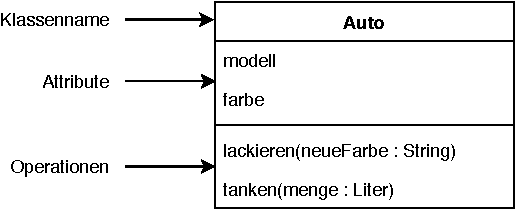
\includegraphics{../grafiken/Kapitel-3/Abb-3-11.pdf}
	\caption{Eine Klasse Auto mit Attributen und Operationen}
	\label{fig:Abb-3-11}
	\vspace{-6pt}
\end{wrapfigure}
Die Nachricht des Sender-Objektes besteht aus einem Operationsnamen und gegebenenfalls zusätzlichen Informationen in Form von Parametern. Das Empfänger-Objekt kann auf diese Nachricht genau dann reagieren, wenn eine entsprechende Operation definiert ist.\footnote{Objektorientierte Programmiersprachen verlangen in der Regel, dass nur Nachrichten gesendet werden, auf die ein Objekt auch reagieren kann. In compilierten Sprachen achtet darauf schon der Compiler. In Interpreter-Sprachen lösen solche Nachrichten Laufzeit-Fehler aus. Der Fall, dass ein Objekt eine Nachricht nicht verstehen kann, wird also im Gegensatz zur Realwelt nicht als gültige Möglichkeit angesehen.} Die Ausgestaltung der Operation bestimmt, was genau bei Eintreffen der Nachricht des Sender-Objektes passiert. Die Operationen, die das Verhalten der Objekte bestimmen, sind für alle Instanzen einer Klasse identisch. 
In der UML-Darstellung werden die Operationen dementsprechend auch in der Klasse notiert und nicht in den einzelnen Instanzen. Dafür wird das Rechteck der Klasse erneut horizontal unterteilt (Abb.~\ref{fig:Abb-3-11}).

Wie bei der Notation der Attribute kann die Angabe von Operationen in UML-Klassendiagrammen je nach Einsatzzweck des Modells mehr oder weniger detailliert sein. Ergänzend zu der minimalen Darstellung in Form des Operationsnamens können auch Eingangs- und/oder Rückgabeparameter oder auch zusätzliche textuelle Erläuterungen zu Implementierungserfordernissen mit angegeben werden. Für die Abbildung des Realwelt-Ausschnittes auf ein Domänenklassendiagramm genügen in der Regel die Operationsnamen.

Jede Instanz bietet genau die in ihrer Klasse definierten Operationen an. Die Reaktion auf einen entsprechenden Operationsaufruf kann aber (und wird meistens) abhängig vom Zustand der Instanz, auf der der Operationsaufruf durchgeführt wird sowie abhängig von den durch das aufrufende Objekt übergebenen Parametern unterschiedlich ausfallen. 
So ist es zum Beispiel sinnvoll, wenn eine Auto-Instanz, deren Tank leer ist, auf den Operationsaufruf tanken(30 Liter) anders reagiert als eine andere Auto-Instanz, deren Tank komplett gefüllt ist. Die Operationen, die ein Objekt anbietet, greifen daher in der Regel auf seine aktuellen Attributwerte zu. Man unterscheidet Operationen, die nur lesend auf Attribute zugreifen und deren Werte nicht verändern (Selektoren) und solche, die Attributwerte verändern, also (auch) schreibend auf Attribute zugreifen (Modifikatoren). Modifikatoren ändern also den Zustand eines Objektes, Selektoren tun dies nicht. Die Operation \texttt{lackieren(neueFarbe: String)} der Klasse \texttt{Auto} in Abbildung~\ref{fig:Abb-3-11} ist ein Beispiel für einen Modifikator, wenn wir sie so entwerfen, dass sie den Wert des Attributs \texttt{farbe} durch den Wert des übergebenen Parameters \texttt{neueFarbe} ersetzt. 
\begin{wrapfigure}{o}[70pt]{0.6\textwidth}
	%\vspace{-10pt}
	\centering 
	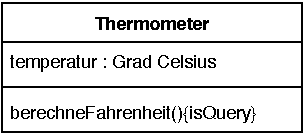
\includegraphics{../grafiken/Kapitel-3/Abb-3-12.pdf}
	\caption{Eine Klasse \texttt{Thermometer} mit Attribut und Selektor-Operation}
	\label{fig:Abb-3-12}
	\vspace{-6pt}
\end{wrapfigure}
Abbildung~\ref{fig:Abb-3-12} zeigt ein Beispiel für eine Selektor-Operation: Die Klasse \texttt{Thermometer} besitzt ein Attribut \texttt{temperatur}, das die Temperatur in der Einheit Grad Celsius enthält. Die Methode \texttt{berechneFahrenheit()} liest diesen Wert aus und errechnet daraus die Temperatur in der Einheit Grad Fahrenheit. In der UML können Selektor-Methoden über den Zusatz \{isQuery\} gekennzeichnet werden. Dieser Zusatz ist aber optional. Für viele Modellierungszwecke im Laufe der Softwareentwicklung ist es nicht relevant, ob eine bestimmte Operation in der späteren konkreten Implementierung ein Selektor oder ein Modifikator werden soll.

Die „einfachsten“ Selektor- und Modifikator-Operationen sind die (eingedeutscht so genannten) Getter und Setter. 
\begin{wrapfigure}{o}[70pt]{0.6\textwidth}
	%\vspace{-10pt}
	\centering 
	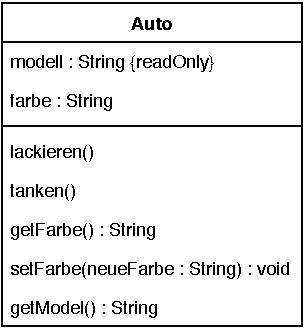
\includegraphics{../grafiken/Kapitel-3/Abb-3-13.pdf}
	\caption{Eine Klasse \texttt{Auto} mit get- und set-Operationen}
	\label{fig:Abb-3-13}
	\vspace{-6pt}
\end{wrapfigure}
Eine get-Operation liest den Wert eines bestimmten Attributes aus und liefert diesen zurück. 
Eine set-Operation nimmt über einen Parameter einen Wert entgegen und ersetzt den aktuellen Wert eines bestimmten Attributes durch den Parameterwert. Es ist üblich, für jedes Attribut der Klasse, auf das auch von außerhalb der Klasse zugegriffen werden soll, get- und set-Operationen in der Klasse zu definieren. Abbildung~\ref{fig:Abb-3-13} zeigt eine Klasse \texttt{Auto} mit einer get- und einer set-Operation für das Attribut \texttt{farbe}. Da das Attribut \texttt{modell} nicht veränderlich sein soll, wird für dieses Attribut nur die get-Operation benötigt. Um ein Klassendiagramm nicht zu überladen, werden die Getter und Setter üblicherweise nicht aufgeführt – auch nicht in sehr implementierungsnahen Klassendiagrammen – sondern erst im Rahmen der konkreten Implementierung erstellt.

Wie bei den Attributen gibt es neben den bisher behandelten Operationen, die jede Instanz der Klasse anbietet, auch explizite Klassenoperationen. Klassenoperationen werden verwendet, um auf die Klassenattribute zuzugreifen. Zudem können sie für Operationen verwendet werden, die sich auf primitive Datentypen beziehen. Primitive Datentypen (in Java zum Beispiel int, boolean, float etc.) sind in den meisten objektorientierten Programmiersprachen keine Objekte und bieten daher auch keine Objektoperationen an. Wie die Klassenattribute werden Klassenoperationen in der UML-Darstellung unterstrichen. 

Eine besondere Form von Operationen sind die Operationen zum Erzeugen und Löschen von Instanzen, die so genannten Konstruktoren und Destruktoren. Wie die Klassenoperationen werden sie unabhängig von einer konkreten Instanz verwendet. In manchen objektorientierten Programmiersprachen entspricht ihre Syntax der Syntax von Klassenoperationen. In Java haben Konstruktoren eine spezielle Syntax, die sich von derjenigen der Klassenoperationen unterscheidet. Zudem kennt Java keine Destruktoren, sondern stattdessen das Konzept des Garbage Collectors.\footnote{zu Konstruktoren, Destruktoren und Garbage Collector vgl. Kurseinheit 5.} Wie die Getter und Setter werden Konstruktoren und Destruktoren aus Übersichtlichkeitsgründen üblicherweise nicht im UML-Klassendiagramm aufgeführt.
